% REDI Architecture Diagram - Compact Version for Two-Column Papers
% For paper: "REDI: Automated Data Readiness for Scientific AI"
%
% This version fits within a single column (~3.5 inches wide)
% Include with: % REDI Architecture Diagram - Compact Version for Two-Column Papers
% For paper: "REDI: Automated Data Readiness for Scientific AI"
%
% This version fits within a single column (~3.5 inches wide)
% Include with: % REDI Architecture Diagram - Compact Version for Two-Column Papers
% For paper: "REDI: Automated Data Readiness for Scientific AI"
%
% This version fits within a single column (~3.5 inches wide)
% Include with: % REDI Architecture Diagram - Compact Version for Two-Column Papers
% For paper: "REDI: Automated Data Readiness for Scientific AI"
%
% This version fits within a single column (~3.5 inches wide)
% Include with: \input{redi_architecture_compact}

\documentclass[tikz,border=5pt]{standalone}
\usepackage{tikz}
\usetikzlibrary{shapes.geometric, arrows.meta, positioning, fit, backgrounds, calc, decorations.pathreplacing}

% Color scheme
\definecolor{rediblue}{RGB}{41, 98, 255}
\definecolor{redipurple}{RGB}{103, 58, 183}
\definecolor{redigreen}{RGB}{0, 150, 136}
\definecolor{rediorange}{RGB}{255, 152, 0}
\definecolor{redigray}{RGB}{96, 125, 139}
\definecolor{lightbg}{RGB}{248, 249, 250}

\begin{document}
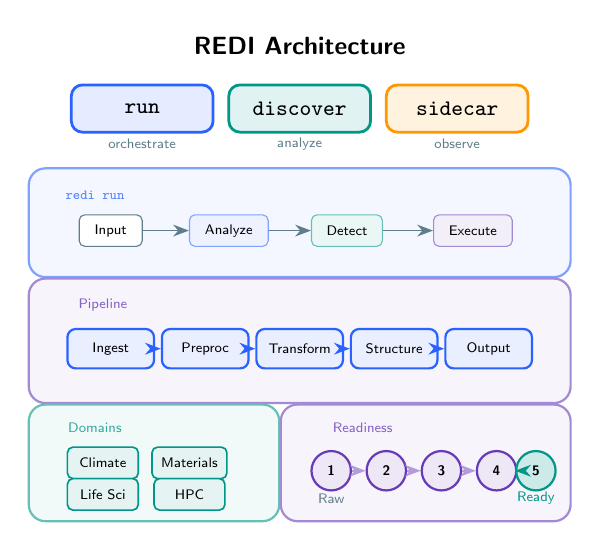
\begin{tikzpicture}[
    node distance=0.3cm,
    mode/.style={
        rectangle, rounded corners=4pt, minimum width=1.8cm, minimum height=0.6cm,
        draw=#1, line width=1pt, fill=#1!12, font=\footnotesize\bfseries\sffamily
    },
    stage/.style={
        rectangle, rounded corners=3pt, minimum width=1.1cm, minimum height=0.5cm,
        draw=rediblue, line width=0.8pt, fill=rediblue!10, font=\tiny\sffamily
    },
    domainnode/.style={
        rectangle, rounded corners=2pt, minimum width=0.9cm, minimum height=0.4cm,
        draw=redigreen, line width=0.6pt, fill=redigreen!10, font=\tiny\sffamily
    },
    level/.style={
        circle, minimum size=0.5cm, draw=redipurple, line width=0.8pt,
        fill=redipurple!12, font=\tiny\bfseries\sffamily
    },
    arrow/.style={->, >=Stealth, line width=0.6pt, color=redigray},
    groupbox/.style={rectangle, rounded corners=6pt, draw=#1!60, line width=0.8pt, fill=#1!5, inner sep=4pt}
]

% ============================================================================
% Title
% ============================================================================
\node[font=\small\bfseries\sffamily] at (0, 5.2) {REDI Architecture};

% ============================================================================
% Three Modes
% ============================================================================
\node[mode=rediblue] (run) at (-2, 4.4) {\texttt{run}};
\node[mode=redigreen] (discover) at (0, 4.4) {\texttt{discover}};
\node[mode=rediorange] (sidecar) at (2, 4.4) {\texttt{sidecar}};

\node[font=\tiny\sffamily, text=redigray] at (-2, 3.95) {orchestrate};
\node[font=\tiny\sffamily, text=redigray] at (0, 3.95) {analyze};
\node[font=\tiny\sffamily, text=redigray] at (2, 3.95) {observe};

% ============================================================================
% Run Mode Flow
% ============================================================================
\begin{scope}[on background layer]
    \node[groupbox=rediblue, fit={($ (-3.3, 3.5) $) ($ (3.3, 2.4) $)}] {};
\end{scope}

\node[font=\tiny\sffamily, text=rediblue!80] at (-2.6, 3.3) {\texttt{redi run}};

% Flow nodes
\node[rectangle, rounded corners=2pt, draw=redigray, fill=white,
      minimum width=0.8cm, minimum height=0.4cm, font=\tiny\sffamily]
      (input) at (-2.4, 2.85) {Input};
\node[rectangle, rounded corners=2pt, draw=rediblue!60, fill=rediblue!8,
      minimum width=1cm, minimum height=0.4cm, font=\tiny\sffamily]
      (analyze) at (-0.9, 2.85) {Analyze};
\node[rectangle, rounded corners=2pt, draw=redigreen!60, fill=redigreen!8,
      minimum width=0.9cm, minimum height=0.4cm, font=\tiny\sffamily]
      (detect) at (0.6, 2.85) {Detect};
\node[rectangle, rounded corners=2pt, draw=redipurple!60, fill=redipurple!8,
      minimum width=1cm, minimum height=0.4cm, font=\tiny\sffamily]
      (exec) at (2.2, 2.85) {Execute};

\draw[arrow] (input) -- (analyze);
\draw[arrow] (analyze) -- (detect);
\draw[arrow] (detect) -- (exec);

% ============================================================================
% 5-Stage Pipeline
% ============================================================================
\begin{scope}[on background layer]
    \node[groupbox=redipurple, fit={($ (-3.3, 2.1) $) ($ (3.3, 0.8) $)}] {};
\end{scope}

\node[font=\tiny\sffamily, text=redipurple!80] at (-2.5, 1.9) {Pipeline};

% Stages
\node[stage] (s1) at (-2.4, 1.35) {Ingest};
\node[stage] (s2) at (-1.2, 1.35) {Preproc};
\node[stage] (s3) at (0, 1.35) {Transform};
\node[stage] (s4) at (1.2, 1.35) {Structure};
\node[stage] (s5) at (2.4, 1.35) {Output};

\draw[arrow, color=rediblue] (s1) -- (s2);
\draw[arrow, color=rediblue] (s2) -- (s3);
\draw[arrow, color=rediblue] (s3) -- (s4);
\draw[arrow, color=rediblue] (s4) -- (s5);

% ============================================================================
% Domains (Left)
% ============================================================================
\begin{scope}[on background layer]
    \node[groupbox=redigreen, fit={($ (-3.3, 0.5) $) ($ (-0.4, -0.7) $)}] {};
\end{scope}

\node[font=\tiny\sffamily, text=redigreen!80] at (-2.6, 0.35) {Domains};

\node[domainnode] (d1) at (-2.5, -0.1) {Climate};
\node[domainnode] (d2) at (-1.4, -0.1) {Materials};
\node[domainnode] (d3) at (-2.5, -0.5) {Life Sci};
\node[domainnode] (d4) at (-1.4, -0.5) {HPC};

% ============================================================================
% Readiness Levels (Right)
% ============================================================================
\begin{scope}[on background layer]
    \node[groupbox=redipurple, fit={($ (-0.1, 0.5) $) ($ (3.3, -0.7) $)}] {};
\end{scope}

\node[font=\tiny\sffamily, text=redipurple!80] at (0.8, 0.35) {Readiness};

\node[level] (l1) at (0.4, -0.2) {1};
\node[level] (l2) at (1.1, -0.2) {2};
\node[level] (l3) at (1.8, -0.2) {3};
\node[level] (l4) at (2.5, -0.2) {4};
\node[level, fill=redigreen!20, draw=redigreen] (l5) at (3.0, -0.2) {5};

\node[font=\tiny\sffamily, text=redigray] at (0.4, -0.55) {Raw};
\node[font=\tiny\sffamily, text=redigreen] at (3.0, -0.55) {Ready};

\draw[arrow, color=redipurple!50] (l1) -- (l2);
\draw[arrow, color=redipurple!50] (l2) -- (l3);
\draw[arrow, color=redipurple!50] (l3) -- (l4);
\draw[arrow, color=redigreen] (l4) -- (l5);

\end{tikzpicture}
\end{document}


\documentclass[tikz,border=5pt]{standalone}
\usepackage{tikz}
\usetikzlibrary{shapes.geometric, arrows.meta, positioning, fit, backgrounds, calc, decorations.pathreplacing}

% Color scheme
\definecolor{rediblue}{RGB}{41, 98, 255}
\definecolor{redipurple}{RGB}{103, 58, 183}
\definecolor{redigreen}{RGB}{0, 150, 136}
\definecolor{rediorange}{RGB}{255, 152, 0}
\definecolor{redigray}{RGB}{96, 125, 139}
\definecolor{lightbg}{RGB}{248, 249, 250}

\begin{document}
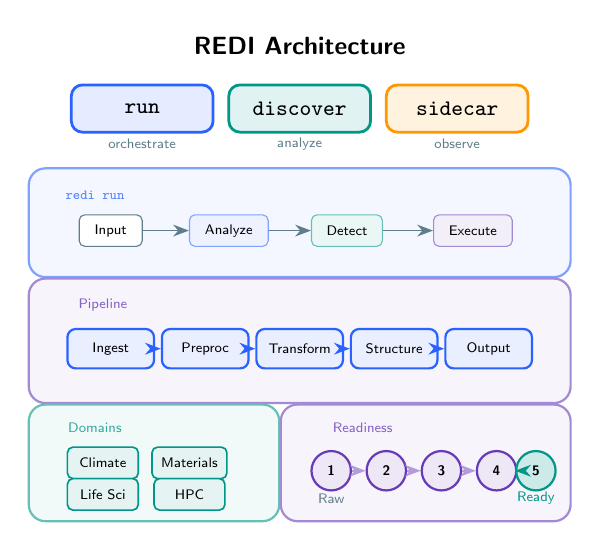
\begin{tikzpicture}[
    node distance=0.3cm,
    mode/.style={
        rectangle, rounded corners=4pt, minimum width=1.8cm, minimum height=0.6cm,
        draw=#1, line width=1pt, fill=#1!12, font=\footnotesize\bfseries\sffamily
    },
    stage/.style={
        rectangle, rounded corners=3pt, minimum width=1.1cm, minimum height=0.5cm,
        draw=rediblue, line width=0.8pt, fill=rediblue!10, font=\tiny\sffamily
    },
    domainnode/.style={
        rectangle, rounded corners=2pt, minimum width=0.9cm, minimum height=0.4cm,
        draw=redigreen, line width=0.6pt, fill=redigreen!10, font=\tiny\sffamily
    },
    level/.style={
        circle, minimum size=0.5cm, draw=redipurple, line width=0.8pt,
        fill=redipurple!12, font=\tiny\bfseries\sffamily
    },
    arrow/.style={->, >=Stealth, line width=0.6pt, color=redigray},
    groupbox/.style={rectangle, rounded corners=6pt, draw=#1!60, line width=0.8pt, fill=#1!5, inner sep=4pt}
]

% ============================================================================
% Title
% ============================================================================
\node[font=\small\bfseries\sffamily] at (0, 5.2) {REDI Architecture};

% ============================================================================
% Three Modes
% ============================================================================
\node[mode=rediblue] (run) at (-2, 4.4) {\texttt{run}};
\node[mode=redigreen] (discover) at (0, 4.4) {\texttt{discover}};
\node[mode=rediorange] (sidecar) at (2, 4.4) {\texttt{sidecar}};

\node[font=\tiny\sffamily, text=redigray] at (-2, 3.95) {orchestrate};
\node[font=\tiny\sffamily, text=redigray] at (0, 3.95) {analyze};
\node[font=\tiny\sffamily, text=redigray] at (2, 3.95) {observe};

% ============================================================================
% Run Mode Flow
% ============================================================================
\begin{scope}[on background layer]
    \node[groupbox=rediblue, fit={($ (-3.3, 3.5) $) ($ (3.3, 2.4) $)}] {};
\end{scope}

\node[font=\tiny\sffamily, text=rediblue!80] at (-2.6, 3.3) {\texttt{redi run}};

% Flow nodes
\node[rectangle, rounded corners=2pt, draw=redigray, fill=white,
      minimum width=0.8cm, minimum height=0.4cm, font=\tiny\sffamily]
      (input) at (-2.4, 2.85) {Input};
\node[rectangle, rounded corners=2pt, draw=rediblue!60, fill=rediblue!8,
      minimum width=1cm, minimum height=0.4cm, font=\tiny\sffamily]
      (analyze) at (-0.9, 2.85) {Analyze};
\node[rectangle, rounded corners=2pt, draw=redigreen!60, fill=redigreen!8,
      minimum width=0.9cm, minimum height=0.4cm, font=\tiny\sffamily]
      (detect) at (0.6, 2.85) {Detect};
\node[rectangle, rounded corners=2pt, draw=redipurple!60, fill=redipurple!8,
      minimum width=1cm, minimum height=0.4cm, font=\tiny\sffamily]
      (exec) at (2.2, 2.85) {Execute};

\draw[arrow] (input) -- (analyze);
\draw[arrow] (analyze) -- (detect);
\draw[arrow] (detect) -- (exec);

% ============================================================================
% 5-Stage Pipeline
% ============================================================================
\begin{scope}[on background layer]
    \node[groupbox=redipurple, fit={($ (-3.3, 2.1) $) ($ (3.3, 0.8) $)}] {};
\end{scope}

\node[font=\tiny\sffamily, text=redipurple!80] at (-2.5, 1.9) {Pipeline};

% Stages
\node[stage] (s1) at (-2.4, 1.35) {Ingest};
\node[stage] (s2) at (-1.2, 1.35) {Preproc};
\node[stage] (s3) at (0, 1.35) {Transform};
\node[stage] (s4) at (1.2, 1.35) {Structure};
\node[stage] (s5) at (2.4, 1.35) {Output};

\draw[arrow, color=rediblue] (s1) -- (s2);
\draw[arrow, color=rediblue] (s2) -- (s3);
\draw[arrow, color=rediblue] (s3) -- (s4);
\draw[arrow, color=rediblue] (s4) -- (s5);

% ============================================================================
% Domains (Left)
% ============================================================================
\begin{scope}[on background layer]
    \node[groupbox=redigreen, fit={($ (-3.3, 0.5) $) ($ (-0.4, -0.7) $)}] {};
\end{scope}

\node[font=\tiny\sffamily, text=redigreen!80] at (-2.6, 0.35) {Domains};

\node[domainnode] (d1) at (-2.5, -0.1) {Climate};
\node[domainnode] (d2) at (-1.4, -0.1) {Materials};
\node[domainnode] (d3) at (-2.5, -0.5) {Life Sci};
\node[domainnode] (d4) at (-1.4, -0.5) {HPC};

% ============================================================================
% Readiness Levels (Right)
% ============================================================================
\begin{scope}[on background layer]
    \node[groupbox=redipurple, fit={($ (-0.1, 0.5) $) ($ (3.3, -0.7) $)}] {};
\end{scope}

\node[font=\tiny\sffamily, text=redipurple!80] at (0.8, 0.35) {Readiness};

\node[level] (l1) at (0.4, -0.2) {1};
\node[level] (l2) at (1.1, -0.2) {2};
\node[level] (l3) at (1.8, -0.2) {3};
\node[level] (l4) at (2.5, -0.2) {4};
\node[level, fill=redigreen!20, draw=redigreen] (l5) at (3.0, -0.2) {5};

\node[font=\tiny\sffamily, text=redigray] at (0.4, -0.55) {Raw};
\node[font=\tiny\sffamily, text=redigreen] at (3.0, -0.55) {Ready};

\draw[arrow, color=redipurple!50] (l1) -- (l2);
\draw[arrow, color=redipurple!50] (l2) -- (l3);
\draw[arrow, color=redipurple!50] (l3) -- (l4);
\draw[arrow, color=redigreen] (l4) -- (l5);

\end{tikzpicture}
\end{document}


\documentclass[tikz,border=5pt]{standalone}
\usepackage{tikz}
\usetikzlibrary{shapes.geometric, arrows.meta, positioning, fit, backgrounds, calc, decorations.pathreplacing}

% Color scheme
\definecolor{rediblue}{RGB}{41, 98, 255}
\definecolor{redipurple}{RGB}{103, 58, 183}
\definecolor{redigreen}{RGB}{0, 150, 136}
\definecolor{rediorange}{RGB}{255, 152, 0}
\definecolor{redigray}{RGB}{96, 125, 139}
\definecolor{lightbg}{RGB}{248, 249, 250}

\begin{document}
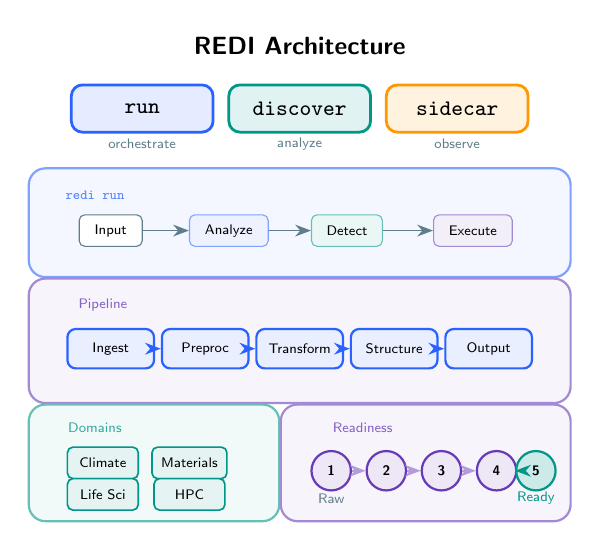
\begin{tikzpicture}[
    node distance=0.3cm,
    mode/.style={
        rectangle, rounded corners=4pt, minimum width=1.8cm, minimum height=0.6cm,
        draw=#1, line width=1pt, fill=#1!12, font=\footnotesize\bfseries\sffamily
    },
    stage/.style={
        rectangle, rounded corners=3pt, minimum width=1.1cm, minimum height=0.5cm,
        draw=rediblue, line width=0.8pt, fill=rediblue!10, font=\tiny\sffamily
    },
    domainnode/.style={
        rectangle, rounded corners=2pt, minimum width=0.9cm, minimum height=0.4cm,
        draw=redigreen, line width=0.6pt, fill=redigreen!10, font=\tiny\sffamily
    },
    level/.style={
        circle, minimum size=0.5cm, draw=redipurple, line width=0.8pt,
        fill=redipurple!12, font=\tiny\bfseries\sffamily
    },
    arrow/.style={->, >=Stealth, line width=0.6pt, color=redigray},
    groupbox/.style={rectangle, rounded corners=6pt, draw=#1!60, line width=0.8pt, fill=#1!5, inner sep=4pt}
]

% ============================================================================
% Title
% ============================================================================
\node[font=\small\bfseries\sffamily] at (0, 5.2) {REDI Architecture};

% ============================================================================
% Three Modes
% ============================================================================
\node[mode=rediblue] (run) at (-2, 4.4) {\texttt{run}};
\node[mode=redigreen] (discover) at (0, 4.4) {\texttt{discover}};
\node[mode=rediorange] (sidecar) at (2, 4.4) {\texttt{sidecar}};

\node[font=\tiny\sffamily, text=redigray] at (-2, 3.95) {orchestrate};
\node[font=\tiny\sffamily, text=redigray] at (0, 3.95) {analyze};
\node[font=\tiny\sffamily, text=redigray] at (2, 3.95) {observe};

% ============================================================================
% Run Mode Flow
% ============================================================================
\begin{scope}[on background layer]
    \node[groupbox=rediblue, fit={($ (-3.3, 3.5) $) ($ (3.3, 2.4) $)}] {};
\end{scope}

\node[font=\tiny\sffamily, text=rediblue!80] at (-2.6, 3.3) {\texttt{redi run}};

% Flow nodes
\node[rectangle, rounded corners=2pt, draw=redigray, fill=white,
      minimum width=0.8cm, minimum height=0.4cm, font=\tiny\sffamily]
      (input) at (-2.4, 2.85) {Input};
\node[rectangle, rounded corners=2pt, draw=rediblue!60, fill=rediblue!8,
      minimum width=1cm, minimum height=0.4cm, font=\tiny\sffamily]
      (analyze) at (-0.9, 2.85) {Analyze};
\node[rectangle, rounded corners=2pt, draw=redigreen!60, fill=redigreen!8,
      minimum width=0.9cm, minimum height=0.4cm, font=\tiny\sffamily]
      (detect) at (0.6, 2.85) {Detect};
\node[rectangle, rounded corners=2pt, draw=redipurple!60, fill=redipurple!8,
      minimum width=1cm, minimum height=0.4cm, font=\tiny\sffamily]
      (exec) at (2.2, 2.85) {Execute};

\draw[arrow] (input) -- (analyze);
\draw[arrow] (analyze) -- (detect);
\draw[arrow] (detect) -- (exec);

% ============================================================================
% 5-Stage Pipeline
% ============================================================================
\begin{scope}[on background layer]
    \node[groupbox=redipurple, fit={($ (-3.3, 2.1) $) ($ (3.3, 0.8) $)}] {};
\end{scope}

\node[font=\tiny\sffamily, text=redipurple!80] at (-2.5, 1.9) {Pipeline};

% Stages
\node[stage] (s1) at (-2.4, 1.35) {Ingest};
\node[stage] (s2) at (-1.2, 1.35) {Preproc};
\node[stage] (s3) at (0, 1.35) {Transform};
\node[stage] (s4) at (1.2, 1.35) {Structure};
\node[stage] (s5) at (2.4, 1.35) {Output};

\draw[arrow, color=rediblue] (s1) -- (s2);
\draw[arrow, color=rediblue] (s2) -- (s3);
\draw[arrow, color=rediblue] (s3) -- (s4);
\draw[arrow, color=rediblue] (s4) -- (s5);

% ============================================================================
% Domains (Left)
% ============================================================================
\begin{scope}[on background layer]
    \node[groupbox=redigreen, fit={($ (-3.3, 0.5) $) ($ (-0.4, -0.7) $)}] {};
\end{scope}

\node[font=\tiny\sffamily, text=redigreen!80] at (-2.6, 0.35) {Domains};

\node[domainnode] (d1) at (-2.5, -0.1) {Climate};
\node[domainnode] (d2) at (-1.4, -0.1) {Materials};
\node[domainnode] (d3) at (-2.5, -0.5) {Life Sci};
\node[domainnode] (d4) at (-1.4, -0.5) {HPC};

% ============================================================================
% Readiness Levels (Right)
% ============================================================================
\begin{scope}[on background layer]
    \node[groupbox=redipurple, fit={($ (-0.1, 0.5) $) ($ (3.3, -0.7) $)}] {};
\end{scope}

\node[font=\tiny\sffamily, text=redipurple!80] at (0.8, 0.35) {Readiness};

\node[level] (l1) at (0.4, -0.2) {1};
\node[level] (l2) at (1.1, -0.2) {2};
\node[level] (l3) at (1.8, -0.2) {3};
\node[level] (l4) at (2.5, -0.2) {4};
\node[level, fill=redigreen!20, draw=redigreen] (l5) at (3.0, -0.2) {5};

\node[font=\tiny\sffamily, text=redigray] at (0.4, -0.55) {Raw};
\node[font=\tiny\sffamily, text=redigreen] at (3.0, -0.55) {Ready};

\draw[arrow, color=redipurple!50] (l1) -- (l2);
\draw[arrow, color=redipurple!50] (l2) -- (l3);
\draw[arrow, color=redipurple!50] (l3) -- (l4);
\draw[arrow, color=redigreen] (l4) -- (l5);

\end{tikzpicture}
\end{document}


\documentclass[tikz,border=5pt]{standalone}
\usepackage{tikz}
\usetikzlibrary{shapes.geometric, arrows.meta, positioning, fit, backgrounds, calc, decorations.pathreplacing}

% Color scheme
\definecolor{rediblue}{RGB}{41, 98, 255}
\definecolor{redipurple}{RGB}{103, 58, 183}
\definecolor{redigreen}{RGB}{0, 150, 136}
\definecolor{rediorange}{RGB}{255, 152, 0}
\definecolor{redigray}{RGB}{96, 125, 139}
\definecolor{lightbg}{RGB}{248, 249, 250}

\begin{document}
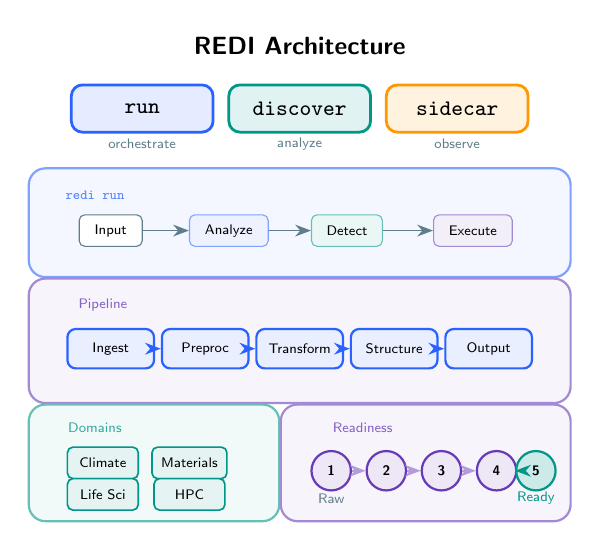
\begin{tikzpicture}[
    node distance=0.3cm,
    mode/.style={
        rectangle, rounded corners=4pt, minimum width=1.8cm, minimum height=0.6cm,
        draw=#1, line width=1pt, fill=#1!12, font=\footnotesize\bfseries\sffamily
    },
    stage/.style={
        rectangle, rounded corners=3pt, minimum width=1.1cm, minimum height=0.5cm,
        draw=rediblue, line width=0.8pt, fill=rediblue!10, font=\tiny\sffamily
    },
    domainnode/.style={
        rectangle, rounded corners=2pt, minimum width=0.9cm, minimum height=0.4cm,
        draw=redigreen, line width=0.6pt, fill=redigreen!10, font=\tiny\sffamily
    },
    level/.style={
        circle, minimum size=0.5cm, draw=redipurple, line width=0.8pt,
        fill=redipurple!12, font=\tiny\bfseries\sffamily
    },
    arrow/.style={->, >=Stealth, line width=0.6pt, color=redigray},
    groupbox/.style={rectangle, rounded corners=6pt, draw=#1!60, line width=0.8pt, fill=#1!5, inner sep=4pt}
]

% ============================================================================
% Title
% ============================================================================
\node[font=\small\bfseries\sffamily] at (0, 5.2) {REDI Architecture};

% ============================================================================
% Three Modes
% ============================================================================
\node[mode=rediblue] (run) at (-2, 4.4) {\texttt{run}};
\node[mode=redigreen] (discover) at (0, 4.4) {\texttt{discover}};
\node[mode=rediorange] (sidecar) at (2, 4.4) {\texttt{sidecar}};

\node[font=\tiny\sffamily, text=redigray] at (-2, 3.95) {orchestrate};
\node[font=\tiny\sffamily, text=redigray] at (0, 3.95) {analyze};
\node[font=\tiny\sffamily, text=redigray] at (2, 3.95) {observe};

% ============================================================================
% Run Mode Flow
% ============================================================================
\begin{scope}[on background layer]
    \node[groupbox=rediblue, fit={($ (-3.3, 3.5) $) ($ (3.3, 2.4) $)}] {};
\end{scope}

\node[font=\tiny\sffamily, text=rediblue!80] at (-2.6, 3.3) {\texttt{redi run}};

% Flow nodes
\node[rectangle, rounded corners=2pt, draw=redigray, fill=white,
      minimum width=0.8cm, minimum height=0.4cm, font=\tiny\sffamily]
      (input) at (-2.4, 2.85) {Input};
\node[rectangle, rounded corners=2pt, draw=rediblue!60, fill=rediblue!8,
      minimum width=1cm, minimum height=0.4cm, font=\tiny\sffamily]
      (analyze) at (-0.9, 2.85) {Analyze};
\node[rectangle, rounded corners=2pt, draw=redigreen!60, fill=redigreen!8,
      minimum width=0.9cm, minimum height=0.4cm, font=\tiny\sffamily]
      (detect) at (0.6, 2.85) {Detect};
\node[rectangle, rounded corners=2pt, draw=redipurple!60, fill=redipurple!8,
      minimum width=1cm, minimum height=0.4cm, font=\tiny\sffamily]
      (exec) at (2.2, 2.85) {Execute};

\draw[arrow] (input) -- (analyze);
\draw[arrow] (analyze) -- (detect);
\draw[arrow] (detect) -- (exec);

% ============================================================================
% 5-Stage Pipeline
% ============================================================================
\begin{scope}[on background layer]
    \node[groupbox=redipurple, fit={($ (-3.3, 2.1) $) ($ (3.3, 0.8) $)}] {};
\end{scope}

\node[font=\tiny\sffamily, text=redipurple!80] at (-2.5, 1.9) {Pipeline};

% Stages
\node[stage] (s1) at (-2.4, 1.35) {Ingest};
\node[stage] (s2) at (-1.2, 1.35) {Preproc};
\node[stage] (s3) at (0, 1.35) {Transform};
\node[stage] (s4) at (1.2, 1.35) {Structure};
\node[stage] (s5) at (2.4, 1.35) {Output};

\draw[arrow, color=rediblue] (s1) -- (s2);
\draw[arrow, color=rediblue] (s2) -- (s3);
\draw[arrow, color=rediblue] (s3) -- (s4);
\draw[arrow, color=rediblue] (s4) -- (s5);

% ============================================================================
% Domains (Left)
% ============================================================================
\begin{scope}[on background layer]
    \node[groupbox=redigreen, fit={($ (-3.3, 0.5) $) ($ (-0.4, -0.7) $)}] {};
\end{scope}

\node[font=\tiny\sffamily, text=redigreen!80] at (-2.6, 0.35) {Domains};

\node[domainnode] (d1) at (-2.5, -0.1) {Climate};
\node[domainnode] (d2) at (-1.4, -0.1) {Materials};
\node[domainnode] (d3) at (-2.5, -0.5) {Life Sci};
\node[domainnode] (d4) at (-1.4, -0.5) {HPC};

% ============================================================================
% Readiness Levels (Right)
% ============================================================================
\begin{scope}[on background layer]
    \node[groupbox=redipurple, fit={($ (-0.1, 0.5) $) ($ (3.3, -0.7) $)}] {};
\end{scope}

\node[font=\tiny\sffamily, text=redipurple!80] at (0.8, 0.35) {Readiness};

\node[level] (l1) at (0.4, -0.2) {1};
\node[level] (l2) at (1.1, -0.2) {2};
\node[level] (l3) at (1.8, -0.2) {3};
\node[level] (l4) at (2.5, -0.2) {4};
\node[level, fill=redigreen!20, draw=redigreen] (l5) at (3.0, -0.2) {5};

\node[font=\tiny\sffamily, text=redigray] at (0.4, -0.55) {Raw};
\node[font=\tiny\sffamily, text=redigreen] at (3.0, -0.55) {Ready};

\draw[arrow, color=redipurple!50] (l1) -- (l2);
\draw[arrow, color=redipurple!50] (l2) -- (l3);
\draw[arrow, color=redipurple!50] (l3) -- (l4);
\draw[arrow, color=redigreen] (l4) -- (l5);

\end{tikzpicture}
\end{document}
